% ****** Start of file apssamp.tex ******
%
%   This file is part of the APS files in the REVTeX 4.2 distribution.
%   Version 4.2a of REVTeX, December 2014
%
%   Copyright (c) 2014 The American Physical Society.
%
%   See the REVTeX 4 README file for restrictions and more information.
%
% TeX'ing this file requires that you have AMS-LaTeX 2.0 installed
% as well as the rest of the prerequisites for REVTeX 4.2
%
% See the REVTeX 4 README file
% It also requires running BibTeX. The commands are as follows:
%
%  1)  latex apssamp.tex
%  2)  bibtex apssamp
%  3)  latex apssamp.tex
%  4)  latex apssamp.tex
%
\documentclass[%
 reprint,
%superscriptaddress,
%groupedaddress,
%unsortedaddress,
%runinaddress,
%frontmatterverbose, 
%preprint,
%preprintnumbers,
%nofootinbib,
%nobibnotes,
%bibnotes,
 amsmath,amssymb,
 aps,
% pra,
% prb,
% rmp,
% prstab,
% prstper,
%floatfix,
]{revtex4-2}

\usepackage{graphicx}% Include figure files
\usepackage{dcolumn}% Align table columns on decimal point
% \usepackage{bm}% bold math
% \usepackage{commath}
\usepackage[hidelinks]{hyperref}
\usepackage{cleveref}
\usepackage{float}
\usepackage{lipsum}

% \usepackage{wrapfig}
% \usepackage[font=small,labelfont=bf]{caption}
% \usepackage{subcaption}
% \usepackage{color}
% \usepackage{listings}
% \usepackage{tabularx}
% \usepackage{svg}
% \usepackage{mhchem}
% \usepackage{tikz}
% \usetikzlibrary{matrix, positioning}

%\usepackage[mathlines]{lineno}% Enable numbering of text and display math
%\linenumbers\relax % Commence numbering lines

\usepackage[%showframe,%Uncomment any one of the following lines to test 
% scale=0.7, marginratio={1:1, 2:3}, ignoreall,% default settings
% text={7in,10in},centering,
margin=1.5cm,
% total={6.5in,8.75in}, top=1.2in, left=0.9in, includefoot,
% height=10in,a5paper,hmargin={3cm,0.8in},
]{geometry}

\begin{document}

% \preprint{APS/123-QED}

\title{Percolation Theory: an Investigation}% Force line breaks with \\

\author{Oliver Dudgeon}
\author{Joseph Parker}
\author{Adam Shaw}

\date{\today}

\begin{abstract}
Percolation theory investigates the properties of randomly generated clusters of objects. Objects are placed with a probability $p$. We focus on the 2D square lattice --- other layouts have been investigated elsewhere. We determine a value for the critical probability of a 2D lattice using a numerical simulation and created a forest fire model on a square lattice which turned out to have the same critical probability.
\end{abstract}

\maketitle

\section{Introduction}

\begin{figure}
    \centering
    \fbox{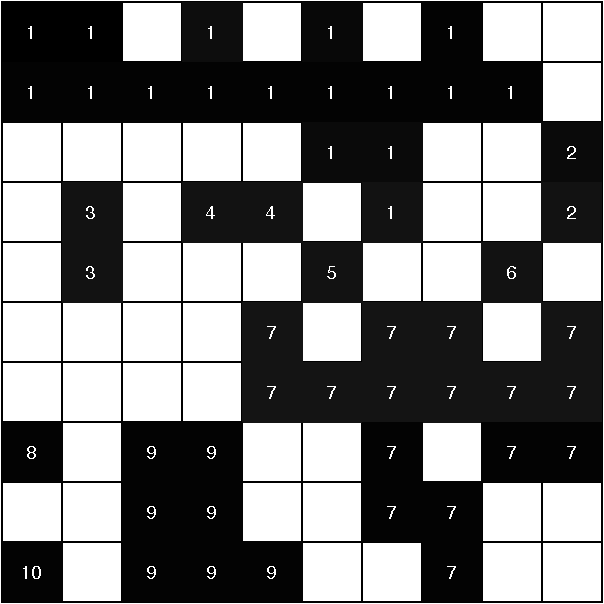
\includegraphics[width=0.7\linewidth]{report/assets/grid.pdf}}
    \caption{A 10 by 10 square lattice. Occupied sites are filled. The number in each site corresponds to the cluster the site is a member of. }
    \label{fig:2D_lat}
\end{figure}

One representation of clustering is that of the 2D square lattice as shown in \cref{fig:2D_lat}. It is often useful to analyse the number of clusters, the sizes of clusters and the shapes of clusters. It is also possible that a cluster spans the entire space. This means there is a cluster for which one can construct a path from one side of the grid to the opposite side of the grid without leaving the original cluster. This is interesting since it implies that the cluster sizes have reached some critical point. It can imply that for an infinitely sized grid there is an infinitely large cluster. 

Although at first glance this can seem like a mathematical interest with little practical use, this model is used in the study of statistical mechanics including the Ising model; disorder in superconductors \cite{alexander_superconductivity_1983} and epidemic modelling including the COVID-19 pandemic \cite{mello_epidemics_2020}.

In this article we restrict ourselves to the 2D lattice. The article is structured as follows. First we develop the methods of two models. Firstly, \cref{sec:site} describes a model of site percolation on a 2D lattice and secondly, \cref{sec:ff} describes a model of forest fires. 

% \subsection{Structure}

% \begin{itemize}
%     \item Generic description of perc theory \cite{stauffer_introduction_2003} y
%     \item Site and Bond percolation y
%     \item Areas where it's used y
%     \begin{itemize}
%         \item Epidemic models (COVID-19) \cite{mello_epidemics_2020} y
%         \item Ising model --- Magnetic systems y
%         \item disorder in superconductors  y
%         \item diluted magnetic semiconductors
%         \item traffic network y
%     \end{itemize}
%     \item Why investigate further
%     \item Report structure
% \end{itemize}

\section{Models}\label{sec:models}
\subsection{Site percolation on a 2D lattice}\label{sec:site}
For a finite 2D lattice, where sites are filled with a probability $p$, there exists a critical probability($p_{c}$) at which you are more likely to find a cluster that spans the grid than you are to not find one. Around this point there are few properties that we can explore, such as phase changes and critical exponents that describe the asymptotic behaviour.

To generate these grids, for each site, we generate a random number between 0 and 1. If the number is less than $p$, then we fill the site i.e. set it to 1 in an array (0 would mean empty).

The critical value $p_{c}$ has different meanings for infinite and finite grids. For infinite grids above $p_{c}$ you will definitely see an infinite cluster appearing --- by definition. For finite grids above $p_{c}$ you are more likely to find a grid where the sites connect two sides than one where they don't.

To analyse the properties of these clusters we would like to know which sites belong to which cluster, from this we can extract the rest of the information we want. Two sites are said to be connected when they share a common edge, this restricts each site to having four neighbours. Knowing this allows us to use a clustering algorithm called the Hoshen-Kopelman algorithm \cite{hoshen_percolation_1976} (HK algorithm), it has a computational complexity of $\mathcal{O}(n)$. 
On the first run, it sweeps through the grid from left to right then top to bottom, for each site it checks the left and top neighbour. If the two sites are empty then a new cluster is created. For one neighbour, the site joins the cluster that the neighbour belongs to. Finally for two neighbours they will both already have cluster numbers, which are not necessarily the same hence we need to link them together. After this we go over the grid again linking all the clusters together so that they have incremental labels. The algorithm is outlined in this flow chart\cref{fig:hk_flow}. Running the HK on the grid in \cref{fig:2D_lat} gives you the labels that are present in the figure.

\begin{figure}
    \centering
    \fbox{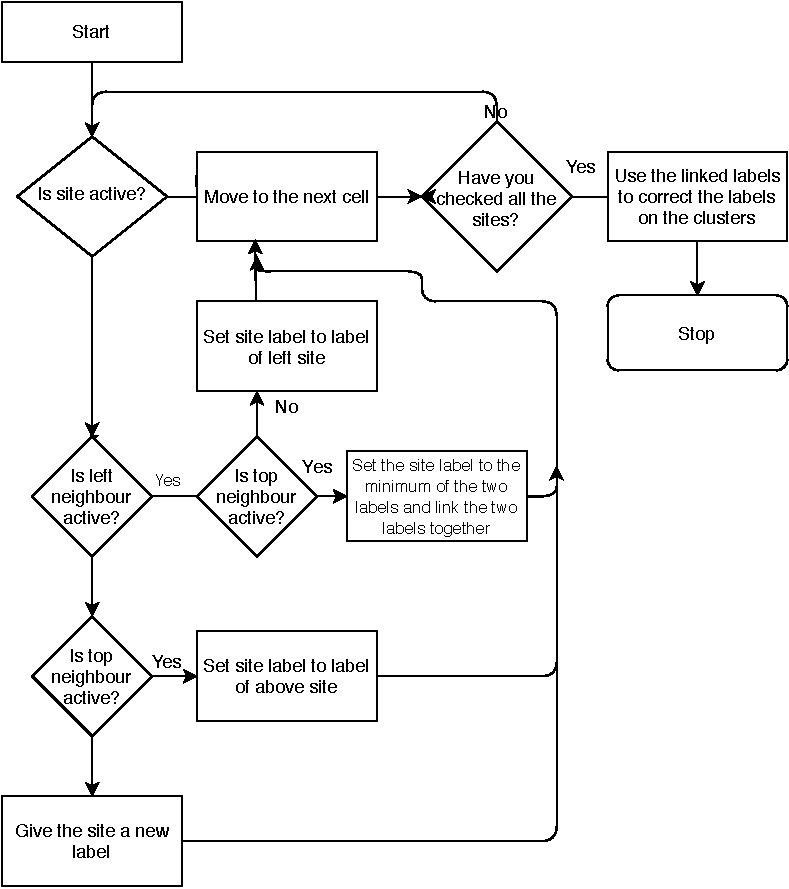
\includegraphics[width=\linewidth]{report/assets/hk_algroithm.pdf}}
    \caption{Hoshen-Kopelman algorithm flow chart. This iterates through the sites labelling each site with the cluster it belongs to. }
    \label{fig:hk_flow}
\end{figure}

For our results we first decided to optimise this algorithm by making use of multiple processing cores. To do this we chose to run the HK algorithm on a different core for each grid. Our hardware limited the number of grids we could run and the size of the grid, due to limited memory. It decreased the time it took for our programs by $30$ times. Normally computing a larger grid size is preferable, in this case you would split up the grid into smaller sub grids then run each sub grid on a separate core. Then you recombine them again into the original grid. This allows you to analyse far greater grid sizes, depending on the number of processing cores and memory you have available.

For our program we used an optimised version of HK, implemented in SciPy's ndimage package\cite{scipy_community_multidimensional_nodate}. This uses a binary tree data structure to reduce the number of neighbours you have to check for each node. It reduced the time for our programs to run by 300 times.
\cite{wu_optimizing_2005}

To find the critical probability for a finite grid, we need a method for detecting clusters that span the grid. This is simple after running the HK algorithm, we only need to check if any labels appear on opposite sides, once we've found a label that does we can say there's a spanning cluster. To find where the critical probability lies one can employ a binary search to converge upon it. A binary search involves keeping track of the upper and lower bounds of $p_{c}$, then using their mean to generate a grid. If the grid has a spanning cluster, we know our $p >= p_{c}$ so we can decrease the upper bound to this value. If there isn't a spanning grid then we increase the lower bound to this value as $p < p_{c}$. Running this until the difference between the bounds is bellow a decided tolerance will give you a numerical result for $p_{c}$. However the problem with this method is that our grids are finite, meaning we can get a spanning cluster bellow $p_{c}$, this will cause the algorithm to not converge exactly to the value of $p_{c}$. Making the grid bigger will reduce the probability of this happening hence giving us more accurate results.

% To analyse the critical point we can look at the behaviour of certain properties around it. The order parameter, $P$, for 2D percolation is the probability of a site being in the infinite cluster. This has the property that is it zero below $p_{c}$ and rises monotonically after. It's equivalent to the density in a liquid-gas system and the magnetisation in magnetic system\cite{yeomans_statistical_1992}. Near the critical point one can show that $P \sim |p-p_{c}|^{\beta}$ near $p_{c}$. The $\beta$ is the critical exponent and used to define equivalence classes for different systems.
% Another property to look at is the cluster number distribution $n(p)$, this gives the number of clusters in a grid built with probability $p$. It can be defined by $n(p) = \sum_{s=0}^{\infty} n_{s}(p)$, where $n_{s}(p)$ is the number of clusters containing $s$ sites at $p$. The critical behaviour for $n_{s}(p_{c})$ only depends on the size of the clusters and not the probability, hence $n_{s}(p_{c}) \sim s^{-\tau}$\cite{stauffer_introduction_2003}, again $\tau$ plays a role in defining equivalence classes. Finding the value of these two parameters is useful for describing the behaviour of the system as you get close to the critical.

\subsection{Forest Fire Model}\label{sec:ff}
% \begin{itemize}
% \item Theory for critical points
% \end{itemize}
The forest fire model is a dynamic percolating system which can be made to exhibit many of the same features as square site percolation\cite{stauffer_introduction_2003}. The attraction of studying the forest fire model is that we can often understand those features in a more intuitive way. 

A grid is randomly populated with trees, each of which may at any time spontaneously catch fire with probability $p_F$. If a tree is adjacent to a fire then the fire spreads to the tree; the original fire then burns itself out, leaving an empty site. We may also introduce a probability for spontaneous tree growth, $p_G$. As long as $p_G$ and $p_F$ are both nonzero, the system will continue to evolve indefinitely. However, a natural way in which to study the behaviour of the system is to define circumstances that cause the simulation to end, and measure the time taken for the system to reach that end\cite{stauffer_introduction_2003}.

In our forest fire model, we defined a $180\times180$ grid of zeros, each representing an empty site. We then randomly turned fraction $p_T$ of those zeros into ones, representing trees. Once this initial grid was produced, our algorithm iteratively passed through the the grid, turning zeros to ones with probability $p_G$, turning ones to twos with probability \(p_F\), turning ones to twos wherever adjacent to an existing two, and turning existing twos into zeros.

This produced a pretty animation, but to perform more quantitative analysis of the system we had to alter some of its characteristics. We chose a simple model where the entire top row of the grid is initially on fire, and both of $p_G$ and $p_F$ are set to zero. The simulation was allowed to proceed until either the fire ran out of new trees to burn, or the fire spread all the way to the bottom row of the grid (i.e. we had a percolating cluster of fire), and we recorded the number of iterations required to reach an end, $t$. We ran the algorithm for multiple initial tree coverage fractions, $p_T$, and repeated the entire process multiple times. Finally, we calculated the mean $t$ for each $p_T$, plotted $t$ against $p_T$, and looked for critical behaviour.
\section{Results}

\subsection{Site}

\begin{figure}
    \centering
    \fbox{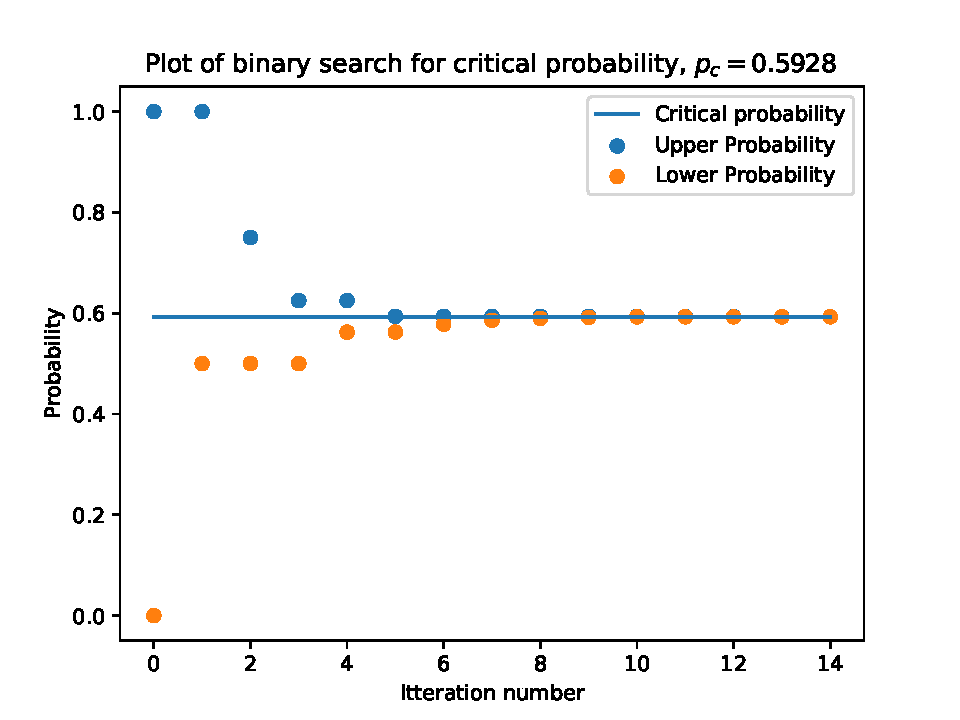
\includegraphics[width=\linewidth]{report/assets/critical_prob.pdf}}
    \caption{Convergence of binary search for critical probability in 2D site percolation, for a square grid with side length $40,000$}
    \label{fig:site_critical_point}
\end{figure}

We ran the binary search method on a 40,000 by 40,000 grid (this size was due to the memory limit of our hardware) with the tolerance on the bounds being $\Delta p \leq 1\times 10^{-4}$. The data is shown in \cref{fig:site_critical_point}

This gave us $p_{c} = 0.5929 \pm 3.1\times10^{-5}$. This is 0.02\% out from the value that Jacobsen found of $p_c =  0.59274...$\cite{Jacobsen_2015}. The true value is out side our error, but this is likely because our grid wasn't big enough. Grids up to $640,000$ width have been simulated before which has 256 times more particles than the one we used \cite{rapaport_multi-million_1991}, if we were able to run ones that size we would be able to obtain a closer value.

% For the $\tau$ exponent we plotted the log of $n_{s}$ vs the log of $s$ of a grid near the critical probability, $p = p_{c} + 0.035$, being to close to $p_{c}$ gives you an incorrect result( as well as being to far away but that's because we are not on an infinite grid)\cite{stauffer_introduction_2003}.

% \begin{figure}
%     \centering
%     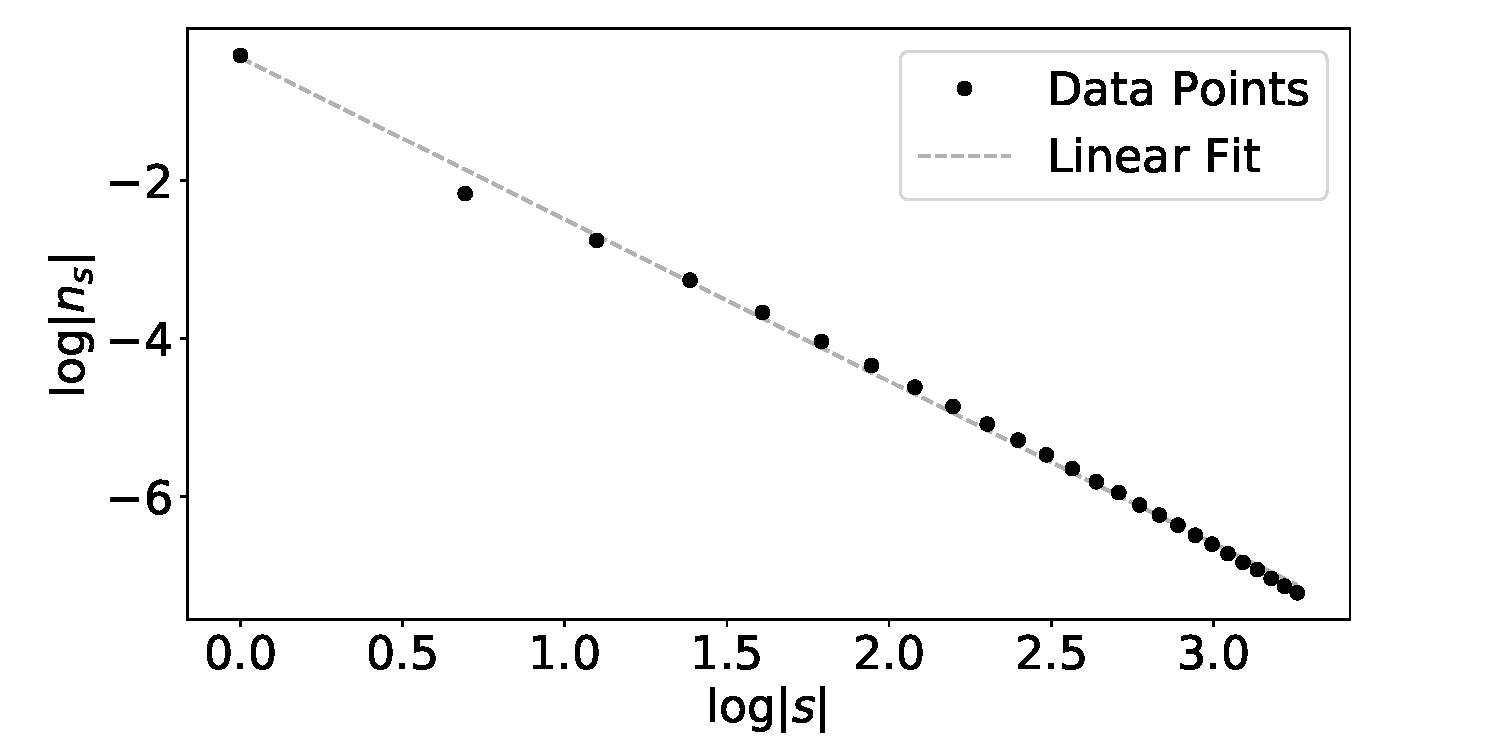
\includegraphics[width=\linewidth]{report/assets/tau_graph.pdf}
%     \caption{Log-log plot of cluster number vs size of cluster for $p \approx p_{c} + 0.035$, with a grid of width 40,000, ignoring smaller clusters.}
% \end{figure}

% We know that $n_{s} \sim s^{-\tau}$ for large s values, so the gradient of our graph will be $-\tau$, this gives us a value $\tau = 2.0470^{+0.0004}_{-0.001}$, the true value is $\tau = 187/91$. Our value for the 40,000 width grid is 0.39\% from the true value.

\subsection{Forest Fire Model}
Plots of the number of iterations before the simulation ended, against initial tree coverage probability, are shown in \cref{fig:FF_mean} and \cref{fig:FF_rawdata}. The plots diverge at a probability of approximately 0.6, with is consistent with our critical probability for square site percolation.
\begin{figure}
    \centering
    \fbox{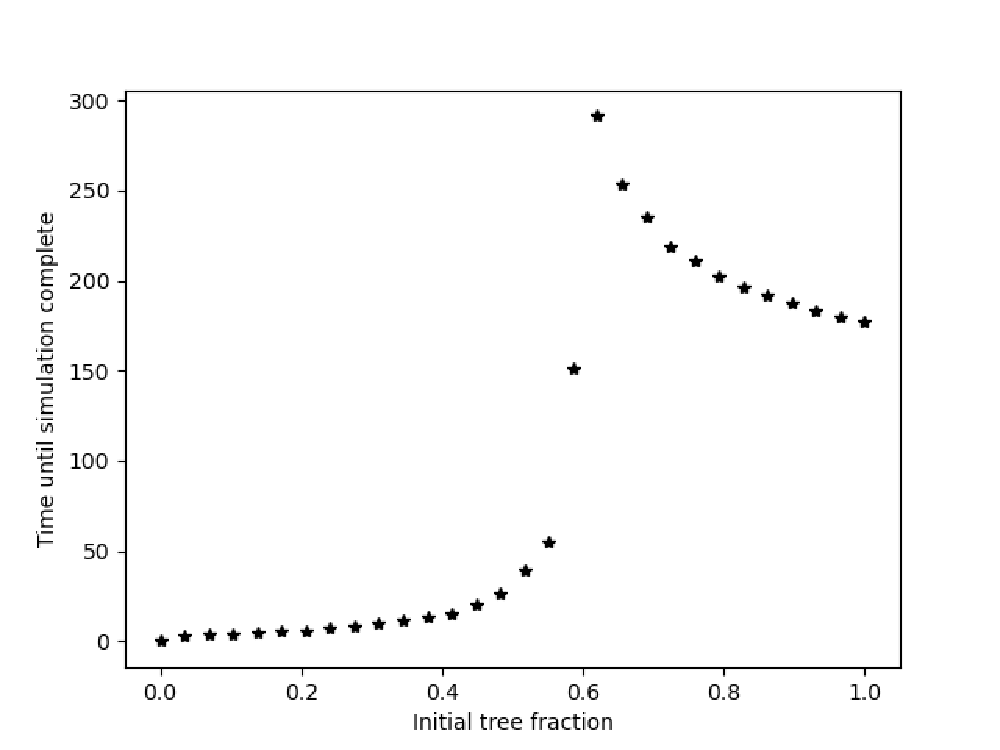
\includegraphics[width=\linewidth]{report/assets/FF_mean_30probs_20reps.pdf}}
    \caption{Number of iterations needed for forest fire simulation to end, plotted against initial tree probabilities. Averaged over 25 runs.}
    \label{fig:FF_mean}
\end{figure}

\begin{figure}
    \centering
    \fbox{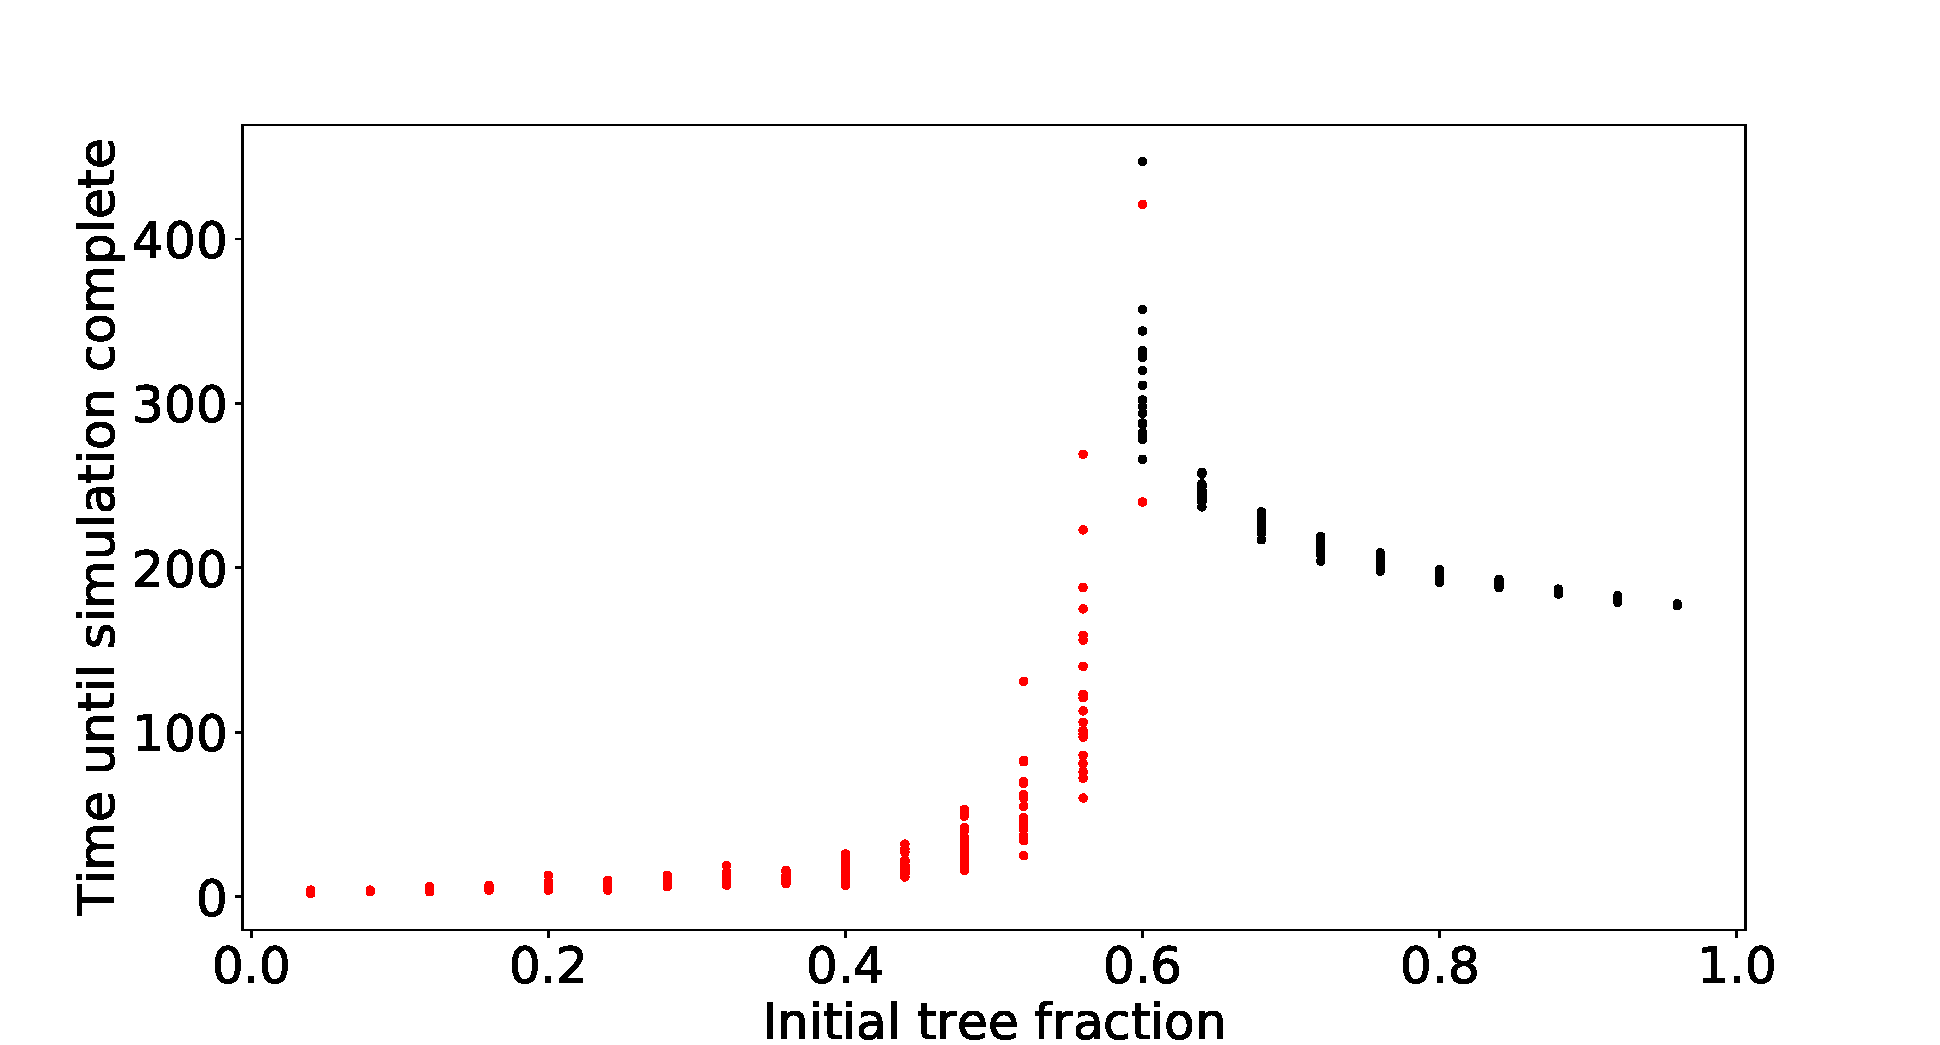
\includegraphics[width=\linewidth]{report/assets/FF_rawdata_25probs_20reps_resize.pdf}}
    \caption{Forest fire iterations vs probabilities, plotted as raw data. Colour indicates the cause of termination.}
    \label{fig:FF_rawdata}
\end{figure}

% \begin{itemize}
% \item Gifs
% \end{itemize}

\section{Discussion}
\subsection{Forest Fire Model}
The fact that, with tree growth and spontaneous fires suppressed, our forest fire model had the same critical probability as square site percolation is not particularly surprising. Indeed, if we ignore the mechanics of fire spread and consider the grid at the point of termination, we see that we do in fact have a square site percolation problem, with clusters made of fire. The difference is that instead of randomly specifying a distribution of fire, we specify a distribution of trees, which then dictate the fire spread and the final cluster sizes. Despite this equivalence, the forest fire model is useful in that it makes the nature of the phase transition much more intuitive - the abstract difference between percolating and non-percolating clusters becomes obvious when we consider fire to spreading through a forest, and \cref{fig:FF_rawdata} nicely illustrates the kind of immediate qualitative change that we associate with phase transitions. 

It is interesting to consider the order parameter of a forest fire simulation. Expanding on the similarity to square site percolation, it seems natural to define the forest fire order parameter as the probability of a site belonging to a fire that cuts all the way through the forest. Just above the critical probability we expect the percolating fire to be as small as possible; for a grid of length $L$ the smallest fire spanning from top to bottom has area $L\delta$, where $\delta$ is some small but finite width. So, as the tree coverage probability $p$ tends to critical probability $p_c$ from above, the order parameter tends to $L\delta/L^2 = \delta/L$, which is always greater than zero. However, as $p\to p_c$ from below, there is no percolating fire, and the order parameter is zero. There is, therefore, a discontinuity in the order parameter at $p_c$ for any finite $L$, meaning that for any finite grid we have a first-order phase transition. However, the discontinuity disappears if we let $L\to\infty$, so an infinite grid would have a second-order phase transition. 

This apparent contradiction disappears if we remember that $p_c$ itself is not well-defined for a finite grid; this is why infinite grids are always used in theoretical work. On the other hand, no physical lattice is ever infinite, so it is interesting to consider the blurred distinction between first and second-order phase transitions in a large, but finite, percolating lattice.

\section{Conclusion}
% Reference GitHub?
\newpage
\bibliography{apssamp}% Produces the bibliography via BibTeX.

\end{document}
%
% ****** End of file apssamp.tex ******
